%physical principles

\section{physical principles}
\subsection{Gamma Decay and Gamma radiation}
Nuclei in excited states can spontaneously transition to lower energy states by emitting a photon (spontaneous emission) or by transferring their energy directly to a shell electron (inner conversion). The Inverse is also possible: if a nucleus is hit by photon that carries the amount energy of a nuclear transition it can be absorbed. The nucleus enters the excited state.

\subsection{Interaction of Gamma radiation with matter}
\begin{figure}[hb]
\centering
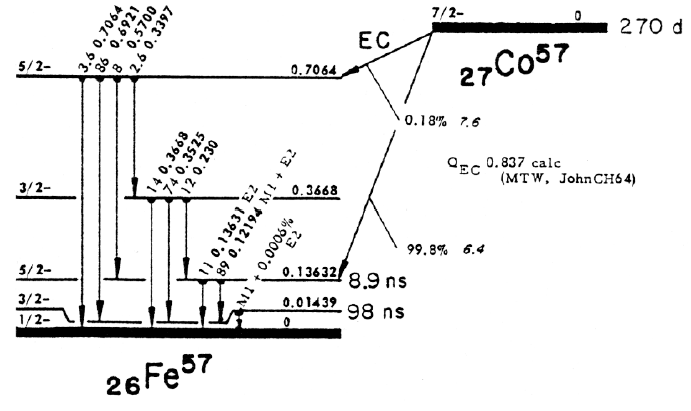
\includegraphics[width=1.0\linewidth]{C:/Users/benjamin/Documents/FPII/Moessbauer/tex/graphics/Zerfallsschema}
\caption[Co-57 decay]{decay series of Cobalt-57}
\label{fig:principles:Zerfallsschema}
\end{figure}
\subsection{Moessbauer effect}

